\chapter{Conclusions and Future Directions}
	
	I began this thesis with a creative interest in computational design, additional interest in digital fabrication, and a personal history of making things by hand. My assumption was that a synthesis of these practices might appeal to other people, especially those who were new to programming. As I complete this thesis and related work, it is clear that  algorithmic craft resonates with many people, from young people, to experienced programmers, to artists and designers. Furthermore, algorithmic craft promotes the values of personal relevance, craftsmanship, beauty, intellectual engagement and pleasure in making. I conclude this thesis with a set of guidelines for tools and practices for future work involving algorithmic craft:
	
		\begin{itemize}
		
		\item \textbf{Tools should support design techniques that demonstrate the benefits of computational design.}  Tools for algorithmic crafting should effectively communicate the affordances of computational design in ways that are accessible to new programmers. This goal can be achieved by providing programming examples that suggest design approaches or by creating built-in programming methods with compelling aesthetic potential.  The radial symmetry algorithms in the DressCode study provide one example. By relying on radial symmetry as a design mechanism, participants were given  a wide range of design possibilities in a format that was relatively easy to understand. Algorithms that produce spirals, waves and basic fractals offer some possibilities for introducing new programmers to computational design. 
				
\item \textbf{The software interface should prioritize interaction through programming.} programming should be the chief method of generating and manipulating designs, and this focus should be reflected in the software interface. The visual design that is produced by the program should be persistent in the software interface and be rapidly updated to reflect changes in the user's code. Additional visual feedback through simulation of a finished artifact is also helpful as in the case of the 3D preview in Codeable Objects. It should be noted that this form of simulation presents a significant technical challenge for complex artifacts.

\item \textbf{Programming languages should have a design-oriented programming syntax, developed with novice programmers in mind.} Algorithmic crafting tools should have a programming syntax and API that is designed to accommodate individuals with no prior programming experience, rather than rely on a general-purpose programming language. The API should be limited to methods and structures relevant to the task of design. By providing users with a small set of useful programming methods that can be used to generate complex forms and patterns, it becomes feasible for novices to engage in intentional and independent computational design.

\item \textbf {Tools should reduce the technical challenges of digital fabrication.} The software should include programming and drawing methods that allow for the production of designs that are suitable for digital fabrication and support for exporting to relevant file formats. The transition from the design tool to the fabrication device should require as few intermediary steps as possible. When possible, it is useful to incorporate methods that give assurance that the design will fabricate as desired. This may include merging all polygons of the same color into one complete path or automatically optimizing lines to increase fabrication speed. 

\item \textbf{Activities should blend domain specificity with creative openness.} Algorithmic craft tools should be able to support numerous creative applications which will encourage the creation of personally relevant, aesthetic outcomes.To encourage the creation of personally relevant aesthetics algorithmic craft tools should be open enough to support numerous creative applications. Algorithmic craft tools should be introduced in a way that provides users with a compelling motivation for their use. For first-time users, algorithmic craft activities should be constrained to the design of a limited set of end products, along with the potential for aesthetic variation. In more general design scenarios, it may be useful to engage designers by asking them to create artifacts that express a specific feeling or emotion, represent a character, or tell a story. Design briefs such as these may further people's inspire awareness of the diverse applications of computational-design and digital fabrication in the realm of self-expression.

\item \textbf{Tools should be supported through fabrication and craft-specific documentation.} In addition to the documentation of the application and programming language, the fabrication and crafting techniques intended for use with the software should be well-documented. This documentation should include an explanation of suitable materials, advice on digital fabrication access, specifications on machine use and settings, and tutorials describing craft components of example projects.

\item \textbf{Activities should encourage discussion and group critiques of work, and when possible, use in-person facilitation and guidance.} Algorithmic craft is a creative practice, not a technical exercise, and as such, it benefits from discussion among peers, critique and reflection. With novice programmers, engagement in these reflective practices is best conducted in a group setting with some form of facilitation. Facilitators can simultaneously provide assistance by addressing coding errors, answering syntax questions, and offering aesthetic design advice. Group algorithmic crafting activities can also provide a casual social atmosphere that is conducive to hand-craft.

\item \textbf{Materials matter.} The use of rich, interesting materials greatly enriches the experience of algorithmic craft and contributes to the success of the finished artifacts. Raw materials like leather, wood, textiles, and art-quality paper complement the precision and complexity of computational design and digital fabrication. Combined in the hands of an engaged user, they can result in objects that are  attractive and durable. Care should also be taken to demonstrate construction techniques that will hold up over time \footnote{Also, if you purchase a large amount of leather, don't leave it near the recycling bin overnight.}.

\item \textbf{ Software tools should be free and open-source.} The software should be freely available and built to function on multiple platforms with low requirements for computational processing power/ These conditions afford high levels of access to casual users. If possible, the software should also be open source in order to encourage the proliferation of additional novice-oriented tools that can be developed for the specific needs of distinct user groups. 

\end{itemize}

\section{Future Directions}

	Many research topics remain to be addressed about  algorithmic  craft.  The software tools that support algorithmic  craft  provide  continued opportunity for innovation. Improvements in  the  ways a tool communicates the  functionality of a program would  improve  the  experience  of the designer  and  the  range  of accomplishments.   Currently,  I am adding a view for declarative design to the DressCode interface that displays a listing of all of the components  in the design (figure:\ref{fig:declarative_view}). The view also shows relationships between groups of objects and their children. This feature  enables a person to manipulate the designs in an imperative form through the programming  interface or by directly  altering  the properties  of individual  primitives  in the declarative view. The choice depends  on what  is most appropriate for the design objective.

 \begin{center}
\begin{figure}[h!]
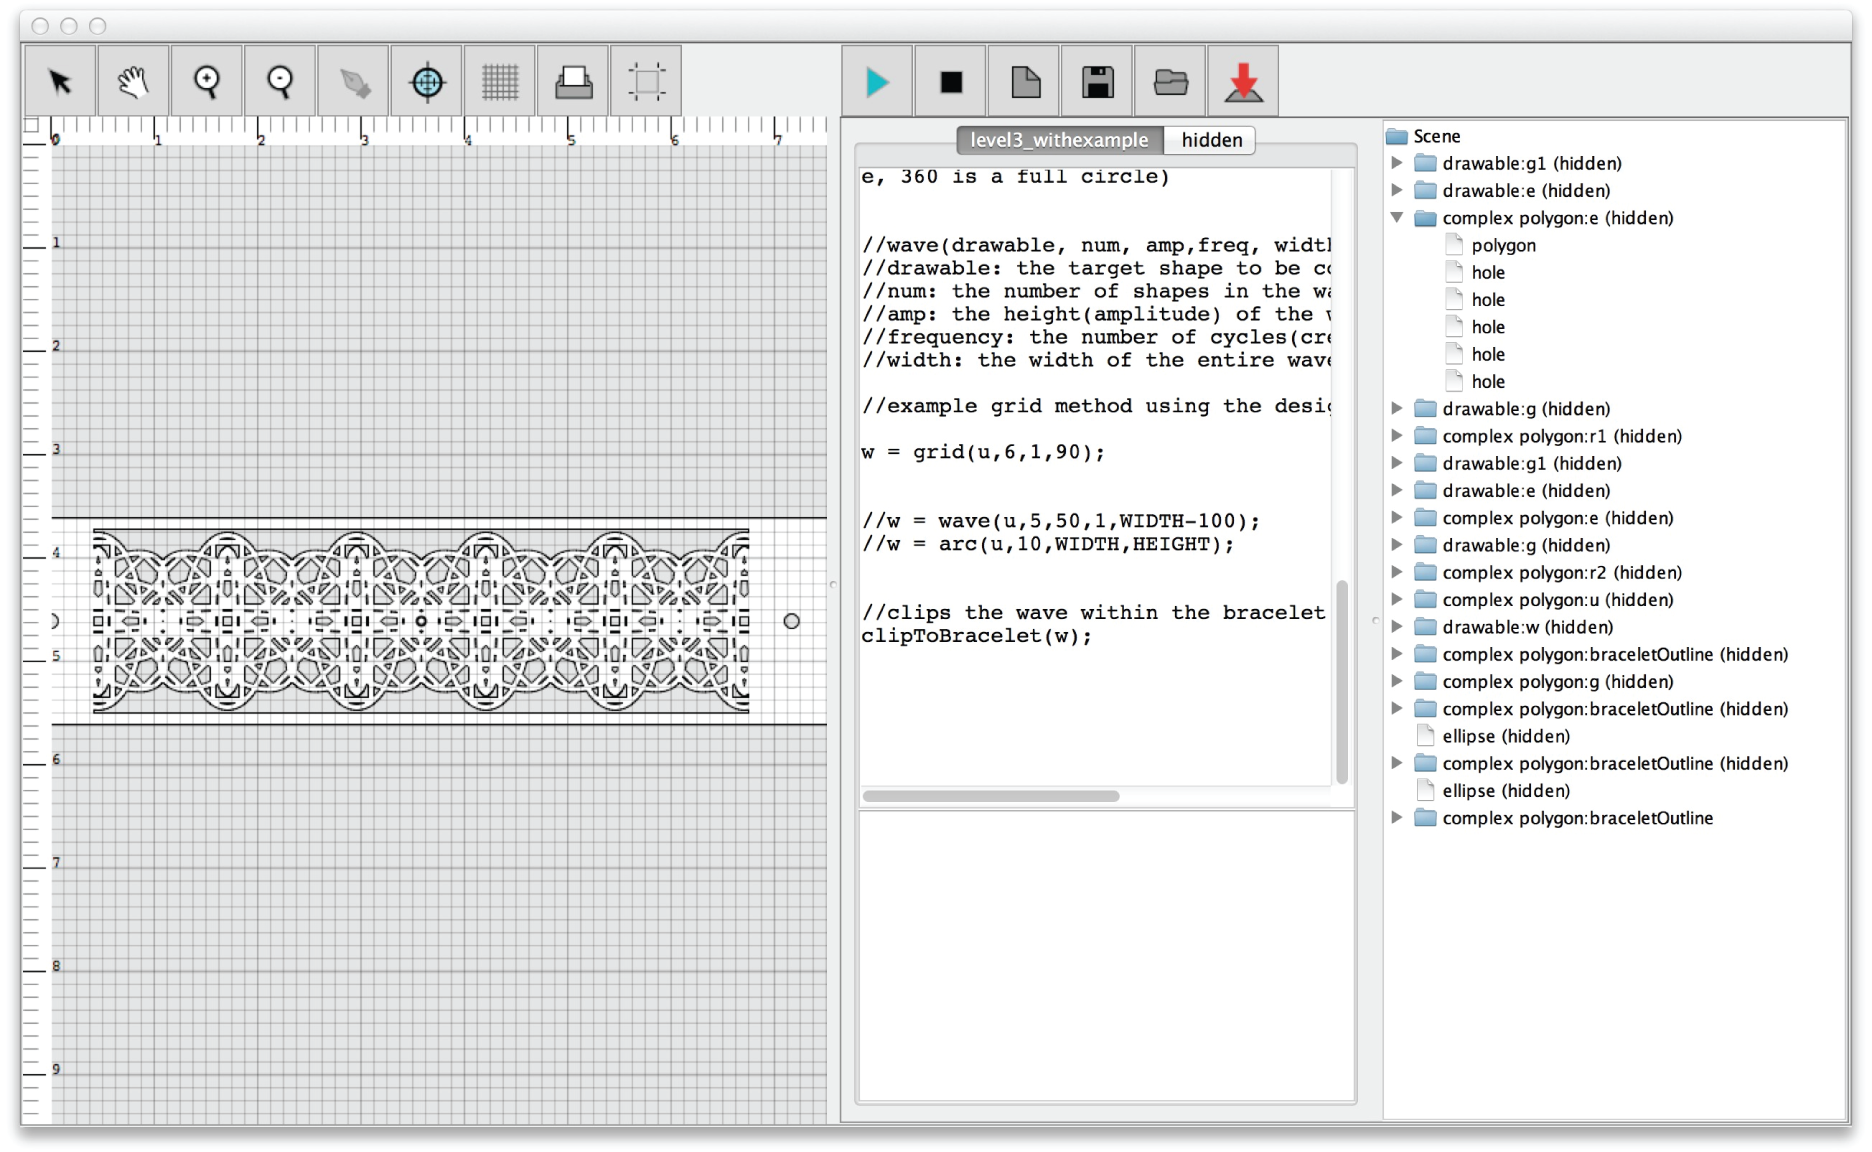
\includegraphics[width=\columnwidth]{images/declarative_view.png}
\caption{DressCode with declarative view of a design}
\label{fig:declarative_view}
\end{figure}
\end{center}

Another important area of future research is the interrelated considerations of maintaining design histories and assisting in design selection. A common challenge of using DressCode is choosing a single design for fabrication  out of numerous possibilities. This issue is not unique to DressCode, but an inherent consideration in computational design. Because algorithmic craft depends on the creation of discrete physical artifacts, design selection in algorithmic craft is more urgent than in screen-based forms of computational design. Future research could explore methods of evaluating numerous designs and providing people with mechanisms for selection. 

Design history is related to design selection. Participants in all of the workshops often created designs that were eventually lost as the participants' code evolved. Participants also often wished to merge components of two separate designs or selectively undo some, but not all, of the changes to a new design. These challenges suggest the need for some form of version control in the software. Version control could not only give people better control of the history of their designs, but also increase the ability to share work, and contribute to the work of others.

Finally, interesting research could be done involving topics of practices and values of craft. Although craft was one of the founding components of this thesis, much of the development time was focused on writing software and learning about the properties of digital fabrication. For future research, I wish to seek the expertise of established craftspeople to improve my understanding of craft practices and how they can be connected to computational design and digital fabrication. One possibility would be to collaborate on the design of a sample tool for algorithmic craft tool with experienced non-digital craftspeople. For example, professional creators of garments or jewelry would be interesting collaborators. They would be knowledgeable in principles of design and product outcomes for their particular fields of practice, but would be novice programmers. This research would allow an analysis of how computational design could be used to augment professional crafting practices. This knowledge could then be used to inform projects and craft strategies for novice crafters. 

\section{Conclusion}
	As computers grow in sophistication, complexity and ubiquity, it becomes possible to regard computation as a disembodied force, outside the reach of most individuals, and incompatible with familiar forms of making. In my experience, the opposite is true. Computers offer potent forms of personal expression by helping us to see the world in new ways. Computation does not invalidate other forms of creation; it enhances them. Computational design, digital fabrication and craft are all special forms of creation. With its generative qualities, computational design can sometimes feel like alchemy. Simple shapes are transmuted to elaborate compositions, almost like magic. Digital fabrication is a way of translating magical computationally-generated forms to physical materials. Craft has a different form of value, a pride in the knowledge that a piece is rare and distinct, and exists as a direct result of the hands that shaped it. By merging these three fields, Algorithmic craft provides people with the opportunity to preserve computational ideas in a individual physical form. As a way of making, algorithmic craft gives people the opportunity to experience the pleasure that is possible when using programming, digital fabrication, and one's hands to build something entirely new. 
	
	
%As computers grow in sophistication, complexity and ubiquity, it becomes possible to regard computation as a disembodied force, outside the reach of most individuals, and incompatible with familiar forms of making. In my experience, the opposite is true. Computers offer potent forms of personal expression by helping us to see the world in new ways. Computation does not invalidate other forms of creation; it enhances them. Algorithmic craft gives people the opportunity to experience the magic and pleasure that is possible when using programming, digital fabrication, and one�s hands to build something entirely new.
	
	